\documentclass[12pt,a4paper,titlepage,final]{article}
% cestina a fonty
\usepackage[czech]{babel}
\usepackage[utf8]{inputenc}
\usepackage[top=2cm, left=1.5cm, text={18cm, 26cm}, ignorefoot]{geometry}
\usepackage{indentfirst}
\usepackage{graphicx}
\usepackage{fancyhdr}
\usepackage{alltt}

\pagestyle{fancy}
\fancyhf{}
\lhead{IIS 2014/15}
\rhead{\textbf{Nejedná se o oficiální materiál!}}
\cfoot{\thepage}

\begin{document}
{ \huge Příprava na IIS semestrálku }

\begin{enumerate}
	{\large \item  Pyramidové schéma}
	\begin{itemize}
		\item \textbf{EIS} -- IS pro exekutivu, pro podporu řízení, k usnadnění a podpoře správy
		\item \textbf{DSS} -- IS pro podporu rozhodování, pro poskytování pomoci při definování a vyhodnocování alternativních akcí
		\item \textbf{MIS} -- IS pro podporu řízení, poskytují informace, které jsou potřebné pro efektivní řízení organizace
		\item \textbf{OLTP} -- IS, které zpracovávají transakčně orientované aplikace
	\end{itemize}
	
	
	{\large \item Definice OLTP jako modelu (asi zobrazení fyzického systému na informační)}
	\begin{itemize}
		\item On-Line Transaction Processing
		\item modeluje nějaký fyzický podsystém
		\item mezi OLTP a jeho fyzickým vzorem existuje izomorfismus
		\item \textbf{Izomorfismus} je zobrazení mezi dvěma matematickými strukturami, které je vzájemně jednoznačné a zachovává všechny vlastnosti touto strukturou definované
	\end{itemize}
	
	
	{\large \item DTD + XSLT na příkladu}
	\begin{verbatim}
Vstup:                                       Výstup:
<priklad>                                    <priklad>
  <hodnota>                                    <hodnota>aaa</hodnota>
    aaa                                        <hodnota>aaa</hodnota>
    <hodnota>                                  <hodnota>bbb</hodnota>
      bbb                                      <hodnota>bbb</hodnota>
      <hodnota>                                <hodnota>ccc</hodnota>
        ccc                                    <hodnota>ccc</hodnota>
      </hodnota>                             </priklad>
    </hodnota>
  </hodnota>
</priklad> 

Řešení DTD:	
<!ELEMENT priklad -- (hodnota) />            <!ELEMENT priklad -- (hodnota*) />
<!ELEMENT hodnota -- (#PCDATA, hodnota?) />  <!ELEMENT hodnota -- (#PCDATA) />

Řešení XSLT:
<xsl:stylesheet version="1.0">
  <xsl:template match="/">
    <xsl:apply-templates select="priklad" />
  </xsl:template>

  <xsl:template match="priklad">
    <priklad>
      <xsl:apply-templates select="hodnota" />
    </priklad>
  </xsl:template>

  <xsl:template match="hodnota">
    <hodnota><xsl:value-of select="text()" /></hodnota>
    <hodnota><xsl:value-of select="text()" /></hodnota>
    <xsl:apply-templates select="hodnota" />
  </xsl:template>
</xsl:stylesheet>
	\end{verbatim}
	
	{\large \item Konzistence transakce}
	\begin{itemize}
		\item návrhář transakce může předpokládat před jejím spuštěním konzistenci databáze
		\item návrhář je ale zodpovědný za zajištění, že po dokončení transakce databáze splňuje všechny integritní omezení a zároveň nový stav modelu odpovídá transformaci, kterou transakce specifikuje
		\item \emph{Transakce je konzistentní, pokud udrží databázi konzistentní a nový databázový stav odpovídá popisu transakce.}
	\end{itemize}
	
	
	{\large \item Zpracováni strukturované transakce, zadaný diagram možných cest z A do E - milníky, nakreslit to co je u příkladu milníku}
   	\begin{verbatim}
                    --( B->C )--
   savepoint1 ---> /            \  <--- obsazený let = rollback1
( T )-->( A->B )--<              >-- ( E )
                   \            /
                    --( B->D )--
   	\end{verbatim}
   	\begin{itemize}
   		\item milník = bod v transakci pro částečný návrat
   		\item používá se částečný návrat \texttt{rollback}
   		\begin{itemize}
   			\item nemění hodnoty v lokálních proměnných	
   			\item pokračuje se za příkazem návratu ve vykonávání transakce
   		\end{itemize}
   		\item musí existovat programový zásobník mílníků, po kterém se v případě rollbacku vracíme
   	\end{itemize}
   	
   	{\large \item Kostka jako svaz kuboidu pro 3 dimenze (misto, cas, zbozi), provést operaci roll-up na nejnižší dimenzi a to namalovat}
   	\begin{figure}[h!]
   		\centering
   		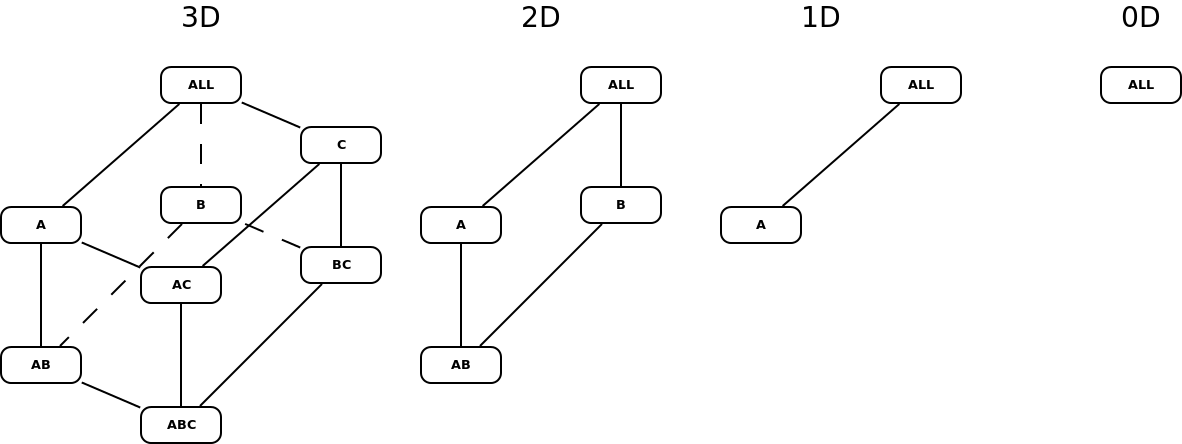
\includegraphics[width=0.9\textwidth]{kostky.png}
   		\caption{Kostka v postupném odrolovávání (A = misto, B = cas, C = zbozi)}
   	\end{figure}
   	
   	Po odrollování na nejnižší dimenzi (0d) nezbyde nic, tedy není co kreslit.
	
	{\large \item Příklad - 2 hierarchicke dimenze - (rok,mesic,den) a (mesto, kraj, stat), 1 fakt - prodejní cena rozhodnout, jestli je to snowflake nebo star a nakreslit schéma }
	
	{\large \item D3, popsat, příklad}
	\begin{itemize}
		\item Data Dependenci Descriptors
		\item definice konzistence je definována množinou \textbf{SUPCA}
		\begin{itemize}
			\item \textbf{S} zdrojový objekt
			\item \textbf{U} cílový objekt, pro změnu hodnoty
			\item \textbf{P} výraz v predikátorovém počtu, který popisuje závislost mezi \textbf{S} a \textbf{U} a nabývá hodnoty true, pokud je pravidlo konzistence splněno
			\item \textbf{C} podmínka určující, kdy musí být dané pravidlo splněno (I-hned, E-v určitou dobu)
			\item \textbf{A} definice algoritmu, který se musí provést, aby predikáty \textbf{P} nabyly hodnoty true	
		\end{itemize}
	\end{itemize}
	
	
	{\large \item Popsat převod M:N vztahu z ER do relační DB}
	\begin{itemize}
		\item vztah M:N není možné převést přímo, ale nutné přidat pomocnou relaci
		\item název je pak složen z názvů obou sloučených entit
		\item jako domény jsou vloženy klíče obou entit
		\item klíč relace je pak složený z klíčů obou entit
	\end{itemize}
	
	{\large \item Popsat application/x-www-form-urlencoded}
	\begin{itemize}
		\item data se píší přímo do URL
		\item oddělována \& a zápis ve tvaru \texttt{<prom>=<hodnota>} 
		\item jako poslední položka je potvrzovací element formuláře a jeho název
		\item \texttt{jmeno=nekdo\&vek=20\&Submit1=Odeslat} 
		\item jdou odesílat \textbf{pouze} string a bool hodnoty
		\item diakritika se musí překodovat do hexa formátu \texttt{\%XX}, kde \texttt{XX} je hexadecimální zápis z ASCII
		\item mezery jsou nahrazovány znakem +
	\end{itemize}
	
	{\large \item Entita v XML, typy }
	\begin{itemize}
		\item možnost fyzicky izolovat a samostatně ukládat libovolnou část dokumentu
		\item každá entita musí být předem deklarovaná
		\item kdy entity používat:
		\begin{itemize}
			\item v případech kdy se stejné informace používají na několika místech == duplikace, vede k chybám
			\item nekompatibilními systémy muže být informace reprezentována špatně
			\item rozsáhlý dokument je vhodné členit	
		\end{itemize}	
		\item klasifikace entit:
		\begin{itemize}
			\item interní a externí
			\item textové a binární	
			\item 4 kombinace, přičemž interní binární kombinace není možná
		\end{itemize}
		
		\item deklarace entity: \texttt{<!ENTITY jmeno entity ...>} 
	\end{itemize}
	
	{\large \item Fragmentace, typy }
	\begin{itemize}
		\item rozdělení relace do několika relací tak, že aktuální relace může být rekonstruována z fragmentů rozptýlených v různých umístěních
		\item dvě základní schémata fragmentace:
		\begin{itemize}
			\item \textbf{horizontální fragmentace:} dělí relaci přiřazením každé n-tice relace $r$ jednomu nebo více fragmentům
			\item \textbf{vertikální fragmentace:} dělí relaci dekompozicí schématu $R$ relace $r$ podle domén	
		\end{itemize}
		\item fragmenty jsou distribuovány v různých uzlech sítě
		\item refragmentace \texttt{union} a \texttt{join} 
	\end{itemize}
	
	{\large \item Pivoting (misto, cas, zbozi) na (cas, zbozi, misto)}
	\begin{figure}[h!]
		\centering
		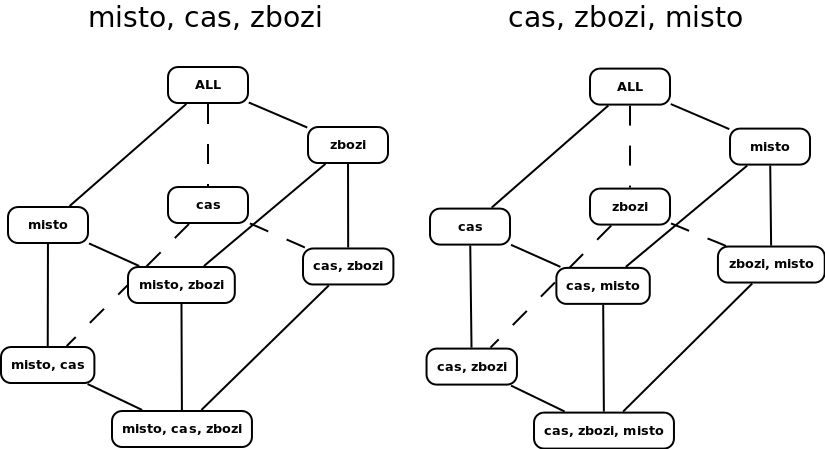
\includegraphics[width=\textwidth]{pivot.png}
		\caption{Pivoting nad 3D kostkou}
	\end{figure}
	
	{\large \item Co je struktura, prostá struktura a objekt}
	\begin{itemize}
		\item \textbf{Struktura:} uspořádané n-tice, které prvky jsou prvky kartouzského součinu jsou strukturované hodnoty vytvářené pevným počtem pojmenovaných dílčích hodnot obecně různých typů
		\item \textbf{Prostá struktura:} struktura bez OID\footnote{Object identification}
		\item \textbf{Objekt:} je struktura s identifikací, je tedy možné jej odkazovat
	\end{itemize}
	
	{\large \item Ve stromové struktuře DOM definovat krátké XML}
	\begin{verbatim}
<book>                                       -> (title = "nazev")
    <title>nazev</title>                   /
    <author>autor</author>          (book) ---> (author = "autor")
    <year>rok</year>                       \
</book>                                      -> (year = "rok")
	\end{verbatim}
	
	{\large \item Vizualizace struktury a kolekce}
	\begin{itemize}
		\item \textbf{Vizualizace kolekce:} 
		\begin{itemize}
			\item Seznam
			\item Tabulka	
		\end{itemize}
		\item \textbf{Vizualizace struktury:} 
		\begin{itemize}
			\item Formulář -- protože položky struktury jsou heterogenní	
		\end{itemize}
	\end{itemize}
	
	{\large \item JSON na XML}
	\begin{verbatim} 
{
  "library": {                        <library>
    "book": [                             <book>
      {                                       <title>neco</title>
        "title": "neco",                      <author>nekdo</author>
        "author": "nekdo"                 </book>
      },                 
      {                                   <book>
        "title": "neco2",                     <title>neco2</title>
        "author": "nekdo2"                    <author>nekdo2</author>
      }                                   </book>
    ]                                 </library>
  }
}
	\end{verbatim}
		
	{\large \item JS na vytažení dat z objektu}
	\begin{verbatim}
		var o = {
		    name:"Nekdo",
		    vek:20
		};
		
		alert(o.name);
		nebo
		alert(o["name"]);
	\end{verbatim}
	
	{\large \item Popsat ACID}
	\begin{itemize}
		\item \textbf{Atomičnost} -- každá transakce je dokončena zcela nebo vůbec
		\item \textbf{Konzistence} -- databázová konzistence
		\item \textbf{Izolovanost} -- souběžné provádění má totožný efekt jako sekvenční
		\item \textbf{Trvanlivost} -- odolnost vůči ztrátě již dokončených změn 	
	\end{itemize}
	
	{\large \item Dědičnost v JavaScriptu}
	\begin{itemize}
		\item provádí se přes \textbf{prototypy} 
	\end{itemize}
	\begin{verbatim}
// konstruktor tridy
function Vozidlo(znacka, spz) {
    this.znacka = znacka;
    this.spz = spz;
}
// konstruktor dedici tridy
function Auto(znacka, spz, barva){
    // volani konstruktoru rodicovske tridy
    this.parent(znacka, spz);
    this.barva = barva;
}
// navazani dedene tridy na rodicovskou
Auto.prototype = Object.create(Vozidlo.prototype);
Auto.prototype.constructor = Auto;
Auto.prototype.parent = Vozidlo;

var moje = new Auto("Skoda", "12345", "cerna");
	\end{verbatim}
	
	{\large \item Asociativní pole X Objekt, napsat JS pro vypis obsahů}
	\begin{verbatim}
// definice pole                          // vypis druheho prvku pole
var pole = [ 1, 2, 3 ];                   alert(pole[1]);
		
// definice objektu
var obj = {                               // vypis vlastnosti a
    a:"aaa";                              alert(obj.a);   
    b:"bbb";                              alert(obj["b"]);
};
	\end{verbatim}
	
	{\large \item Napsat funkci, která bude includovat .js soubory.}
	\begin{verbatim}
var linkgen = function (jmeno) {
    return "<sc"+"ript language='JavaScript' src='"+jmeno+".js"+"'></sc"+"ript>";
}; // linkgen		
	\end{verbatim}
	
\end{enumerate}

\end{document}
